% Options for packages loaded elsewhere
\PassOptionsToPackage{unicode}{hyperref}
\PassOptionsToPackage{hyphens}{url}
\PassOptionsToPackage{dvipsnames,svgnames,x11names}{xcolor}
%
\documentclass[
  letterpaper,
  DIV=11,
  numbers=noendperiod]{scrartcl}

\usepackage{amsmath,amssymb}
\usepackage{iftex}
\ifPDFTeX
  \usepackage[T1]{fontenc}
  \usepackage[utf8]{inputenc}
  \usepackage{textcomp} % provide euro and other symbols
\else % if luatex or xetex
  \usepackage{unicode-math}
  \defaultfontfeatures{Scale=MatchLowercase}
  \defaultfontfeatures[\rmfamily]{Ligatures=TeX,Scale=1}
\fi
\usepackage{lmodern}
\ifPDFTeX\else  
    % xetex/luatex font selection
\fi
% Use upquote if available, for straight quotes in verbatim environments
\IfFileExists{upquote.sty}{\usepackage{upquote}}{}
\IfFileExists{microtype.sty}{% use microtype if available
  \usepackage[]{microtype}
  \UseMicrotypeSet[protrusion]{basicmath} % disable protrusion for tt fonts
}{}
\makeatletter
\@ifundefined{KOMAClassName}{% if non-KOMA class
  \IfFileExists{parskip.sty}{%
    \usepackage{parskip}
  }{% else
    \setlength{\parindent}{0pt}
    \setlength{\parskip}{6pt plus 2pt minus 1pt}}
}{% if KOMA class
  \KOMAoptions{parskip=half}}
\makeatother
\usepackage{xcolor}
\setlength{\emergencystretch}{3em} % prevent overfull lines
\setcounter{secnumdepth}{5}
% Make \paragraph and \subparagraph free-standing
\ifx\paragraph\undefined\else
  \let\oldparagraph\paragraph
  \renewcommand{\paragraph}[1]{\oldparagraph{#1}\mbox{}}
\fi
\ifx\subparagraph\undefined\else
  \let\oldsubparagraph\subparagraph
  \renewcommand{\subparagraph}[1]{\oldsubparagraph{#1}\mbox{}}
\fi

\usepackage{color}
\usepackage{fancyvrb}
\newcommand{\VerbBar}{|}
\newcommand{\VERB}{\Verb[commandchars=\\\{\}]}
\DefineVerbatimEnvironment{Highlighting}{Verbatim}{commandchars=\\\{\}}
% Add ',fontsize=\small' for more characters per line
\usepackage{framed}
\definecolor{shadecolor}{RGB}{241,243,245}
\newenvironment{Shaded}{\begin{snugshade}}{\end{snugshade}}
\newcommand{\AlertTok}[1]{\textcolor[rgb]{0.68,0.00,0.00}{#1}}
\newcommand{\AnnotationTok}[1]{\textcolor[rgb]{0.37,0.37,0.37}{#1}}
\newcommand{\AttributeTok}[1]{\textcolor[rgb]{0.40,0.45,0.13}{#1}}
\newcommand{\BaseNTok}[1]{\textcolor[rgb]{0.68,0.00,0.00}{#1}}
\newcommand{\BuiltInTok}[1]{\textcolor[rgb]{0.00,0.23,0.31}{#1}}
\newcommand{\CharTok}[1]{\textcolor[rgb]{0.13,0.47,0.30}{#1}}
\newcommand{\CommentTok}[1]{\textcolor[rgb]{0.37,0.37,0.37}{#1}}
\newcommand{\CommentVarTok}[1]{\textcolor[rgb]{0.37,0.37,0.37}{\textit{#1}}}
\newcommand{\ConstantTok}[1]{\textcolor[rgb]{0.56,0.35,0.01}{#1}}
\newcommand{\ControlFlowTok}[1]{\textcolor[rgb]{0.00,0.23,0.31}{#1}}
\newcommand{\DataTypeTok}[1]{\textcolor[rgb]{0.68,0.00,0.00}{#1}}
\newcommand{\DecValTok}[1]{\textcolor[rgb]{0.68,0.00,0.00}{#1}}
\newcommand{\DocumentationTok}[1]{\textcolor[rgb]{0.37,0.37,0.37}{\textit{#1}}}
\newcommand{\ErrorTok}[1]{\textcolor[rgb]{0.68,0.00,0.00}{#1}}
\newcommand{\ExtensionTok}[1]{\textcolor[rgb]{0.00,0.23,0.31}{#1}}
\newcommand{\FloatTok}[1]{\textcolor[rgb]{0.68,0.00,0.00}{#1}}
\newcommand{\FunctionTok}[1]{\textcolor[rgb]{0.28,0.35,0.67}{#1}}
\newcommand{\ImportTok}[1]{\textcolor[rgb]{0.00,0.46,0.62}{#1}}
\newcommand{\InformationTok}[1]{\textcolor[rgb]{0.37,0.37,0.37}{#1}}
\newcommand{\KeywordTok}[1]{\textcolor[rgb]{0.00,0.23,0.31}{#1}}
\newcommand{\NormalTok}[1]{\textcolor[rgb]{0.00,0.23,0.31}{#1}}
\newcommand{\OperatorTok}[1]{\textcolor[rgb]{0.37,0.37,0.37}{#1}}
\newcommand{\OtherTok}[1]{\textcolor[rgb]{0.00,0.23,0.31}{#1}}
\newcommand{\PreprocessorTok}[1]{\textcolor[rgb]{0.68,0.00,0.00}{#1}}
\newcommand{\RegionMarkerTok}[1]{\textcolor[rgb]{0.00,0.23,0.31}{#1}}
\newcommand{\SpecialCharTok}[1]{\textcolor[rgb]{0.37,0.37,0.37}{#1}}
\newcommand{\SpecialStringTok}[1]{\textcolor[rgb]{0.13,0.47,0.30}{#1}}
\newcommand{\StringTok}[1]{\textcolor[rgb]{0.13,0.47,0.30}{#1}}
\newcommand{\VariableTok}[1]{\textcolor[rgb]{0.07,0.07,0.07}{#1}}
\newcommand{\VerbatimStringTok}[1]{\textcolor[rgb]{0.13,0.47,0.30}{#1}}
\newcommand{\WarningTok}[1]{\textcolor[rgb]{0.37,0.37,0.37}{\textit{#1}}}

\providecommand{\tightlist}{%
  \setlength{\itemsep}{0pt}\setlength{\parskip}{0pt}}\usepackage{longtable,booktabs,array}
\usepackage{calc} % for calculating minipage widths
% Correct order of tables after \paragraph or \subparagraph
\usepackage{etoolbox}
\makeatletter
\patchcmd\longtable{\par}{\if@noskipsec\mbox{}\fi\par}{}{}
\makeatother
% Allow footnotes in longtable head/foot
\IfFileExists{footnotehyper.sty}{\usepackage{footnotehyper}}{\usepackage{footnote}}
\makesavenoteenv{longtable}
\usepackage{graphicx}
\makeatletter
\def\maxwidth{\ifdim\Gin@nat@width>\linewidth\linewidth\else\Gin@nat@width\fi}
\def\maxheight{\ifdim\Gin@nat@height>\textheight\textheight\else\Gin@nat@height\fi}
\makeatother
% Scale images if necessary, so that they will not overflow the page
% margins by default, and it is still possible to overwrite the defaults
% using explicit options in \includegraphics[width, height, ...]{}
\setkeys{Gin}{width=\maxwidth,height=\maxheight,keepaspectratio}
% Set default figure placement to htbp
\makeatletter
\def\fps@figure{htbp}
\makeatother
% definitions for citeproc citations
\NewDocumentCommand\citeproctext{}{}
\NewDocumentCommand\citeproc{mm}{%
  \begingroup\def\citeproctext{#2}\cite{#1}\endgroup}
\makeatletter
 % allow citations to break across lines
 \let\@cite@ofmt\@firstofone
 % avoid brackets around text for \cite:
 \def\@biblabel#1{}
 \def\@cite#1#2{{#1\if@tempswa , #2\fi}}
\makeatother
\newlength{\cslhangindent}
\setlength{\cslhangindent}{1.5em}
\newlength{\csllabelwidth}
\setlength{\csllabelwidth}{3em}
\newenvironment{CSLReferences}[2] % #1 hanging-indent, #2 entry-spacing
 {\begin{list}{}{%
  \setlength{\itemindent}{0pt}
  \setlength{\leftmargin}{0pt}
  \setlength{\parsep}{0pt}
  % turn on hanging indent if param 1 is 1
  \ifodd #1
   \setlength{\leftmargin}{\cslhangindent}
   \setlength{\itemindent}{-1\cslhangindent}
  \fi
  % set entry spacing
  \setlength{\itemsep}{#2\baselineskip}}}
 {\end{list}}
\usepackage{calc}
\newcommand{\CSLBlock}[1]{\hfill\break\parbox[t]{\linewidth}{\strut\ignorespaces#1\strut}}
\newcommand{\CSLLeftMargin}[1]{\parbox[t]{\csllabelwidth}{\strut#1\strut}}
\newcommand{\CSLRightInline}[1]{\parbox[t]{\linewidth - \csllabelwidth}{\strut#1\strut}}
\newcommand{\CSLIndent}[1]{\hspace{\cslhangindent}#1}

\KOMAoption{captions}{tableheading}
\makeatletter
\@ifpackageloaded{caption}{}{\usepackage{caption}}
\AtBeginDocument{%
\ifdefined\contentsname
  \renewcommand*\contentsname{Table of contents}
\else
  \newcommand\contentsname{Table of contents}
\fi
\ifdefined\listfigurename
  \renewcommand*\listfigurename{List of Figures}
\else
  \newcommand\listfigurename{List of Figures}
\fi
\ifdefined\listtablename
  \renewcommand*\listtablename{List of Tables}
\else
  \newcommand\listtablename{List of Tables}
\fi
\ifdefined\figurename
  \renewcommand*\figurename{Figure}
\else
  \newcommand\figurename{Figure}
\fi
\ifdefined\tablename
  \renewcommand*\tablename{Table}
\else
  \newcommand\tablename{Table}
\fi
}
\@ifpackageloaded{float}{}{\usepackage{float}}
\floatstyle{ruled}
\@ifundefined{c@chapter}{\newfloat{codelisting}{h}{lop}}{\newfloat{codelisting}{h}{lop}[chapter]}
\floatname{codelisting}{Listing}
\newcommand*\listoflistings{\listof{codelisting}{List of Listings}}
\makeatother
\makeatletter
\makeatother
\makeatletter
\@ifpackageloaded{caption}{}{\usepackage{caption}}
\@ifpackageloaded{subcaption}{}{\usepackage{subcaption}}
\makeatother
\ifLuaTeX
  \usepackage{selnolig}  % disable illegal ligatures
\fi
\usepackage{bookmark}

\IfFileExists{xurl.sty}{\usepackage{xurl}}{} % add URL line breaks if available
\urlstyle{same} % disable monospaced font for URLs
\hypersetup{
  pdftitle={The Joyceless Landscape of Stream of Consciousness Literature},
  pdfauthor={Quang Mai},
  colorlinks=true,
  linkcolor={blue},
  filecolor={Maroon},
  citecolor={Blue},
  urlcolor={Blue},
  pdfcreator={LaTeX via pandoc}}

\title{The Joyceless Landscape of Stream of Consciousness
Literature\thanks{Code and data are available at:
https://github.com/ponolite/stream-consciousness-language.git}}
\usepackage{etoolbox}
\makeatletter
\providecommand{\subtitle}[1]{% add subtitle to \maketitle
  \apptocmd{\@title}{\par {\large #1 \par}}{}{}
}
\makeatother
\subtitle{Exploring Word Frequency, Sentiment Value and Mental Health
Themes in the Works of Joyce, Woolf, Proust, Mansfield and Eliot from
Project Gutenberg}
\author{Quang Mai}
\date{April 4, 2024}

\begin{document}
\maketitle
\begin{abstract}
This project focuses on understanding the language used by renowned
stream of consciousness (SOC) authors James Joyce, Virginia Woolf,
Marcel Proust, Katherine Mansfield and T.S Eliot. By conducting word
frequency analysis and sentiment analysis of these authors' nine novels,
I aim to uncover shared linguistic patterns and gain insights into the
authors' mental states. Through the analysis on SOC literature, this
paper thus attempts to offer insights into themes of self-identity,
anxiety, disassociation and existential contemplation within Western
society's from late 19th to mid-20th century. (add one sentence on main
results)
\end{abstract}

\renewcommand*\contentsname{Table of contents}
{
\hypersetup{linkcolor=}
\setcounter{tocdepth}{3}
\tableofcontents
}
\section{Introduction}\label{introduction}

Stream of consciousness (SOC) is a narrative technique that aims to
capture the continuous flow of thoughts, feelings, and sensations
experienced by a character without conventional organization or
punctuation (Bernini and Fernyhough 2022). It mirrors the unpredictable
and interconnected nature of human thought processes, often revealing
the inner workings of the character's mind in an intimate and unfiltered
manner (Long and So 2016). In literature, most scholars agree that
stream of consciousness reveals the complexities of mind-scapes,
shedding light on the nuances of characters' emotional well-being and
psychological struggles (Nyongesa 2023). As such, this paper has mined
the texts of a total of nine novels from the volunteer archive, Project
Gutenberg, to examine the mental health themes of famous stream of
consciousness authors, namely by Joyce, Woolf, Proust, Mansfield and
Eliot, from the modernist era of literature, spanning from late 19th
century to mid-20th century ({``Project Gutenberg,''} n.d.). (more stats
and data mentioned here)

By analyzing these textual datasets through word frequency and sentiment
analysis, I seek to pose and answer crucial questions:
\textit{What are some important factors contributing to this relationship between mental health, disassociation and stream of consciousness? Moreover, how does this relationship vary differently across differnet demographics of authors, for instance, authors with different geographical locations and genders?}
Understanding these dynamics is crucial in having an informed
understanding of the West's late 19th to mid-20th century literature and
even socio-political landscape, especially in regards to how authors and
creative writers navigate and deal with then-taboo topics such as
existential angst, mental health issues and disabilities.

Thus, my estimand is the correlation between mental health-related words
in SOC literature, their frequency and sentimental value as provided by
Mohammad and Turney (2013). This is considered in terms of nine selected
SOC novels only, namely Joyce's A Portrait of the Artist as a Young Man
and Chamber Music; Woolf's Mrs Dalloway and Jacob's Room; Proust's Swann
Way; Mansfield's Bliss and The Garden Party; and Eliot's The Waste Land
and The Love Song of J. Alfred Prufrock. Through our analysis, we found
that (percentage, number and data here, main results)\ldots{}

To further understand the correlation between stream of consciousness
novels and mental health themes, in
\hyperref[introduction]{Introduction}, the paper briefly discusses the
nature of stream of consciousness literature, relevant authors and the
works that I've chosen to analyze. Subsequently, in
\hyperref[sec-data]{Data} and \hyperref[results]{Results}, I talk about
the nature of the data obtained and analyze the results garnered from
the data with suitable tables and charts. Next,
\hyperref[discussion]{Discussion} provides further insights and future
areas of study. Finally, {[}Conclusion{]} summarizes our main findings.
To complete the paper, \hyperref[appendix]{Appendix} clarifies how each
variable within each dataset is generated with relevant tables to
accordingly demonstrate this.

The novel texts used for analysis were sourced from Project Gutenberg
under the library \texttt{gutenbergr} (Johnston and Robinson 2023)
({``Project Gutenberg,''} n.d.). Data was generated, extracted and
cleaned using the open-source statistical programming language R (R Core
Team 2022), leveraging functions from \texttt{tidyverse} (Wickham et al.
2019), \texttt{tidytext} (Julia Silge and Robinson 2016),
\texttt{rmarkdown} (Allaire et al. 2024), \texttt{dplyr} (Wickham et al.
2022), \texttt{ggplot2} (Wickham 2016), \texttt{scales} (Wickham,
Pedersen, and Seidel 2023), \texttt{here} (Müller 2020), \texttt{igraph}
(J. Silge and Robinson 2006), \texttt{widyr} (J. Silge and Robinson
2022), \texttt{ggraph} (Pedersen 2024), \texttt{textdata} (Hvitfeldt
2022), \texttt{tm} (Feinerer, Hornik, and Meyer 2008) and \texttt{knitr}
(Xie 2014).

\section{Data}\label{sec-data}

\subsection{Measurement}\label{measurement}

Two central variables in this paper are:

\begin{itemize}
\tightlist
\item
  \textbf{Word Frequency:} This variable captures the repetition of a
  single word (unigram), two-words combination (bigram) or three-words
  combination (trigram) throughout a SOC novel text, providing us with a
  thematic understanding of SOC literature.
\item
  \textbf{Sentiment Value:} This variable enables us to analyze how
  every word is usually perceived emotionally, whether it be positively
  or negatively. In additon, in childlessness over time, encompassing
  the chosen time frame for the survey.
\end{itemize}

Out of two variables used, the first one, `Word Frequency' usually
captured as \texttt{n} or \texttt{frequency} in datasets, is directly
quantified through tokenizing the novel texts using the packages Julia
Silge and Robinson (2016; Robertson 2021) (Henry 2021). To do this, I
first downloaded all nine novel texts from {``Project Gutenberg''}
(n.d.), and leveraged functions such as \texttt{unnest\_tokens()} from
Julia Silge and Robinson (2016) to mine the texts, or separating it into
individual words. Finally, I used \texttt{count()} to quantify the word
frequency.

The second variable used, `Sentiment Value', is based on three
English-based, general-purpose ``word-emotion and word-polarity
association lexicons'', specifically Mohammad and Turney (2013)'s
expansive research along with efforts from Finn Årup Nielsen and Bing
Liu and collaborators (Julia Silge and Robinson 2016).

The three general-purpose lexicon that contributes to my sentiment
analysis are (Julia Silge and Robinson 2016):

\begin{itemize}[label={$\square$}]
    \item AFINN from Finn Årup Nielsen, which assigns a numerical value from '-5 to 5' 
    \item bing from Bing Liu and collaborators, which assigns if a word is 'positive' or negative'
    \item nrc from Saif Mohammad and Peter Turney, which assigns a core emotional value to a word, such as 'fear', 'anger', 'sadness' or 'trust'.
\end{itemize}

In terms of measuring `Sentiment Value', all three general-purpose
lexicons are compiled through crowd-sourcing and directly surveying the
public on how each word is emotionally perceived

A survey sample of how the word `startle' is compiled within the `nrc'
lexicon is presented below (Mohammad and Turney 2013):

\begin{enumerate}
\def\labelenumi{(\arabic{enumi})}
\tightlist
\item
  Which word is closest in meaning (most related) to startle?
\end{enumerate}

\begin{itemize}
\tightlist
\item
  automobile
\item
  shake
\item
  honesty
\item
  entertain
\end{itemize}

\begin{enumerate}
\def\labelenumi{(\arabic{enumi})}
\setcounter{enumi}{1}
\tightlist
\item
  How positive (good, praising) is the word startle?:
\end{enumerate}

\begin{itemize}
\tightlist
\item
  startle is not positive
\item
  startle is weakly positive
\item
  startle is moderately positive
\item
  startle is strongly positive
\end{itemize}

\begin{enumerate}
\def\labelenumi{(\arabic{enumi})}
\setcounter{enumi}{2}
\tightlist
\item
  How negative (bad, criticizing) is the word startle?
\end{enumerate}

\begin{itemize}
\tightlist
\item
  startle is not negative
\item
  startle is weakly negative
\item
  startle is moderately negativ
\item
  startle is strongly negative
\end{itemize}

After the survey results are garnered, researchers average the answers
to sort each surveyed word into pre-defined categories, specifically `-5
to 5' for `AFINN', `postive' or `negative' for `bing', and `anger' or
`fear' for `nrc'. With the continuous work of compiling these lexicons
spanning years and decades (Mohammad and Turney 2013) comes these
functions: \texttt{get\_sentiments("bing")} and
\texttt{get\_sentiments("nrc")} and \texttt{get\_sentiments("nrc")} in
which I can use \texttt{inner\_join} to categorize my exisitng datasets
of novel texts into existing sentiment value. Systematic and
data-driven, these measurement methods ensure that all lexicons
faithfully reflects each word's emotionality.

However, I do recognize how decontextualized and reductive this
quantification of language can be. When it comes to understand such
social and human artifacts as language or literary texts, much is
dependent on their contextuality. As such, I will further discuss these
weaknesses of the datasets under \hyperref[discussion]{Discussion}.

\subsection{Source Data}\label{source-data}

\subsection{Data Cleaning and Word
Tokenization}\label{data-cleaning-and-word-tokenization}

\begin{table}

\caption{\label{tbl-genderclass}Table of Number of Classes Students
Considered for Regrade Requests by Students' Gender}

\centering{

}

\end{table}%

\subsubsection{Word Count}\label{word-count}

\begin{longtable}[]{@{}
  >{\raggedleft\arraybackslash}p{(\columnwidth - 6\tabcolsep) * \real{0.0988}}
  >{\raggedright\arraybackslash}p{(\columnwidth - 6\tabcolsep) * \real{0.5802}}
  >{\raggedright\arraybackslash}p{(\columnwidth - 6\tabcolsep) * \real{0.1728}}
  >{\raggedright\arraybackslash}p{(\columnwidth - 6\tabcolsep) * \real{0.1481}}@{}}

\caption{\label{tbl-joyce}An Examplary Table Containing Unprocessed
Novel Text (James Joyce)}

\tabularnewline

\toprule\noalign{}
\begin{minipage}[b]{\linewidth}\raggedleft
Book ID
\end{minipage} & \begin{minipage}[b]{\linewidth}\raggedright
Text
\end{minipage} & \begin{minipage}[b]{\linewidth}\raggedright
Book
\end{minipage} & \begin{minipage}[b]{\linewidth}\raggedright
Author
\end{minipage} \\
\midrule\noalign{}
\endhead
\bottomrule\noalign{}
\endlastfoot
2817 & To deep and deeper blue, & Chamber Music & James Joyce \\
2817 & NA & Chamber Music & James Joyce \\
2817 & III At that hour when all things have repose, & Chamber Music &
James Joyce \\
2817 & O lonely watcher of the skies, & Chamber Music & James Joyce \\
2817 & NA & Chamber Music & James Joyce \\

\end{longtable}

\begin{longtable}[]{@{}
  >{\raggedleft\arraybackslash}p{(\columnwidth - 6\tabcolsep) * \real{0.1176}}
  >{\raggedright\arraybackslash}p{(\columnwidth - 6\tabcolsep) * \real{0.5882}}
  >{\raggedright\arraybackslash}p{(\columnwidth - 6\tabcolsep) * \real{0.1765}}
  >{\raggedright\arraybackslash}p{(\columnwidth - 6\tabcolsep) * \real{0.1176}}@{}}

\caption{\label{tbl-joyce-token}An Examplary Table Containing Tokenzied
Novel Text (James Joyce)}

\tabularnewline

\toprule\noalign{}
\begin{minipage}[b]{\linewidth}\raggedleft
Book ID
\end{minipage} & \begin{minipage}[b]{\linewidth}\raggedright
Book
\end{minipage} & \begin{minipage}[b]{\linewidth}\raggedright
Author
\end{minipage} & \begin{minipage}[b]{\linewidth}\raggedright
Word
\end{minipage} \\
\midrule\noalign{}
\endhead
\bottomrule\noalign{}
\endlastfoot
4217 & A Portrait of the Artist as a Young Man & James Joyce & stead \\
4217 & A Portrait of the Artist as a Young Man & James Joyce & dublin \\
4217 & A Portrait of the Artist as a Young Man & James Joyce & 1904 \\
4217 & A Portrait of the Artist as a Young Man & James Joyce &
trieste \\
4217 & A Portrait of the Artist as a Young Man & James Joyce & 1914 \\

\end{longtable}

\newpage

\begin{longtable}[]{@{}lr@{}}

\caption{\label{tbl-joyce-words}An Examplary Table Containing Word Count
of Each Word within Novel Texts (James Joyce)}

\tabularnewline

\toprule\noalign{}
Word & Count \\
\midrule\noalign{}
\endhead
\bottomrule\noalign{}
\endlastfoot
stephen & 373 \\
god & 194 \\
eyes & 180 \\
soul & 178 \\
father & 151 \\

\end{longtable}

\subsubsection{Comparative Word
Frequency}\label{comparative-word-frequency}

\begin{longtable}[]{@{}
  >{\raggedright\arraybackslash}p{(\columnwidth - 10\tabcolsep) * \real{0.1429}}
  >{\raggedleft\arraybackslash}p{(\columnwidth - 10\tabcolsep) * \real{0.1429}}
  >{\raggedleft\arraybackslash}p{(\columnwidth - 10\tabcolsep) * \real{0.2381}}
  >{\raggedleft\arraybackslash}p{(\columnwidth - 10\tabcolsep) * \real{0.1667}}
  >{\raggedleft\arraybackslash}p{(\columnwidth - 10\tabcolsep) * \real{0.1310}}
  >{\raggedleft\arraybackslash}p{(\columnwidth - 10\tabcolsep) * \real{0.1786}}@{}}

\caption{\label{tbl-frequency}Word Frequency of Stream of Consciousness
Novels, A Comparison Between Five Authors}

\tabularnewline

\toprule\noalign{}
\begin{minipage}[b]{\linewidth}\raggedright
Word
\end{minipage} & \begin{minipage}[b]{\linewidth}\raggedleft
James Joyce
\end{minipage} & \begin{minipage}[b]{\linewidth}\raggedleft
Katherine Mansfield
\end{minipage} & \begin{minipage}[b]{\linewidth}\raggedleft
Marcel Proust
\end{minipage} & \begin{minipage}[b]{\linewidth}\raggedleft
T.S. Eliot
\end{minipage} & \begin{minipage}[b]{\linewidth}\raggedleft
Virignia Woolf
\end{minipage} \\
\midrule\noalign{}
\endhead
\bottomrule\noalign{}
\endlastfoot
abandon & 0.000112 & NA & 8.19e-05 & NA & NA \\
abandoned & 0.000112 & NA & 8.19e-05 & NA & NA \\
abandonment & 0.000112 & NA & 8.19e-05 & NA & 0.0001421 \\
abase & 0.000112 & NA & NA & NA & NA \\
abased & 0.000112 & NA & NA & NA & NA \\

\end{longtable}

\subsubsection{Generating Word Networks}\label{generating-word-networks}

\section{Model}\label{model}

The goal of our modelling strategy is twofold. Firstly,\ldots{}

Here we briefly describe the Bayesian analysis model used to
investigate\ldots{} Background details and diagnostics are included in
Appendix~\ref{sec-model-details}.

\subsection{Model set-up}\label{model-set-up}

Define \(y_i\) as the number of seconds that the plane remained aloft.
Then \(\beta_i\) is the wing width and \(\gamma_i\) is the wing length,
both measured in millimeters.

\begin{align} 
y_i|\mu_i, \sigma &\sim \mbox{Normal}(\mu_i, \sigma) \\
\mu_i &= \alpha + \beta_i + \gamma_i\\
\alpha &\sim \mbox{Normal}(0, 2.5) \\
\beta &\sim \mbox{Normal}(0, 2.5) \\
\gamma &\sim \mbox{Normal}(0, 2.5) \\
\sigma &\sim \mbox{Exponential}(1)
\end{align}

We run the model in R (R Core Team 2023) using the \texttt{rstanarm}
package of (\textbf{rstanarm?}). We use the default priors from
\texttt{rstanarm}.

\subsubsection{Model justification}\label{model-justification}

We expect a negative relationship between average household income and
the number of children per child care space by ward. In
particular\ldots{}

We can use maths by including latex between dollar signs, for instance
\(\theta\).

\section{Results}\label{results}

\subsection{The Dominant Vocabulary of SOC
Literature}\label{the-dominant-vocabulary-of-soc-literature}

\begin{figure}

\begin{minipage}{0.50\linewidth}

\centering{

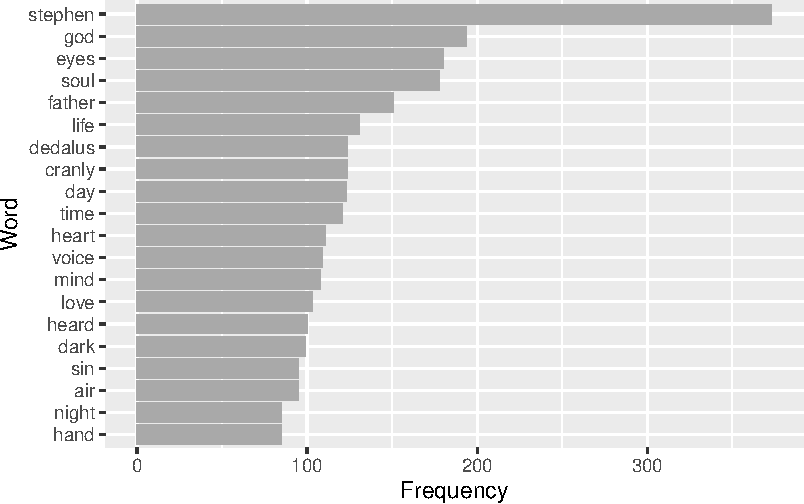
\includegraphics{paper_files/figure-pdf/fig-count-1.pdf}

}

\subcaption{\label{fig-count-1}James Joyce}

\end{minipage}%
%
\begin{minipage}{0.50\linewidth}

\centering{

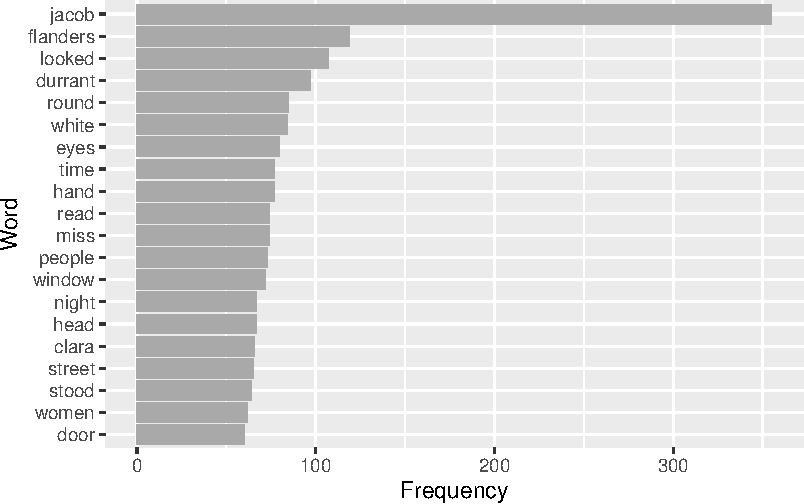
\includegraphics{paper_files/figure-pdf/fig-count-2.pdf}

}

\subcaption{\label{fig-count-2}Virginia Woolf}

\end{minipage}%
\newline
\begin{minipage}{0.50\linewidth}

\centering{

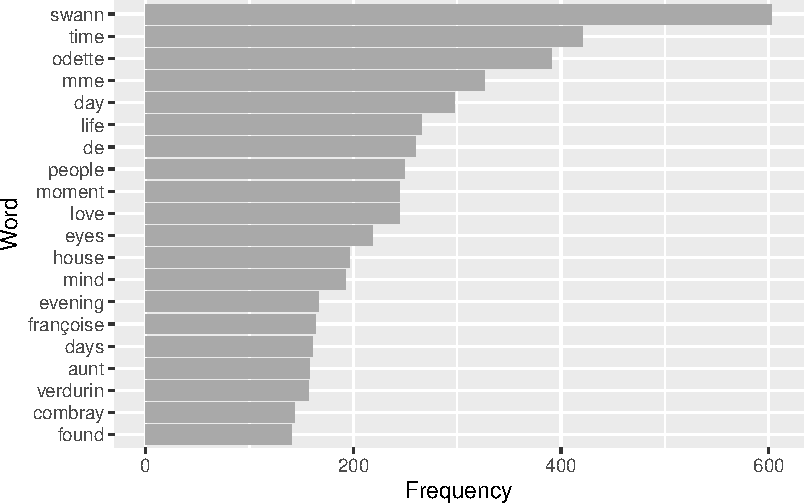
\includegraphics{paper_files/figure-pdf/fig-count-3.pdf}

}

\subcaption{\label{fig-count-3}Marcel Proust}

\end{minipage}%
%
\begin{minipage}{0.50\linewidth}

\centering{

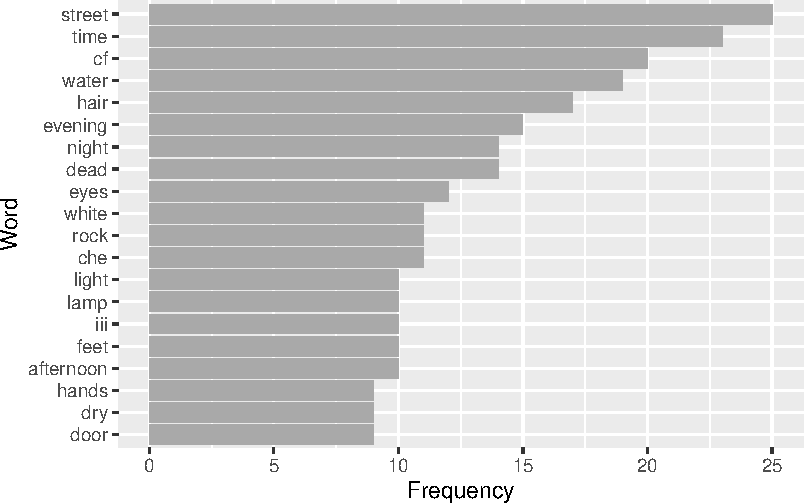
\includegraphics{paper_files/figure-pdf/fig-count-4.pdf}

}

\subcaption{\label{fig-count-4}T.S. Eliot}

\end{minipage}%
\newline
\begin{minipage}{0.50\linewidth}

\centering{

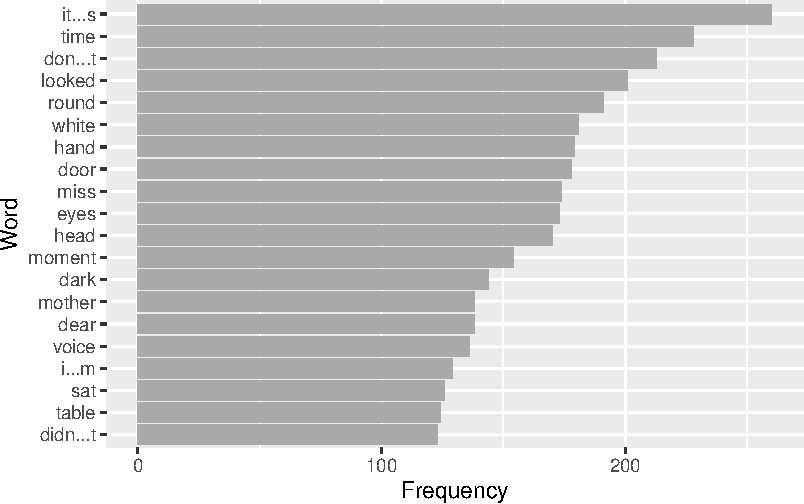
\includegraphics{paper_files/figure-pdf/fig-count-5.pdf}

}

\subcaption{\label{fig-count-5}Katherine Mansfield}

\end{minipage}%

\caption{\label{fig-count}Comparative Analysis of Top 20 Word
Frequencies from Famous SOC Authors}

\end{figure}%

\newpage

\subsection{Sentiment Analysis}\label{sentiment-analysis}

Leveraging setiment analysis from Mohammad and Turney (2013)

\begin{figure}

\centering{

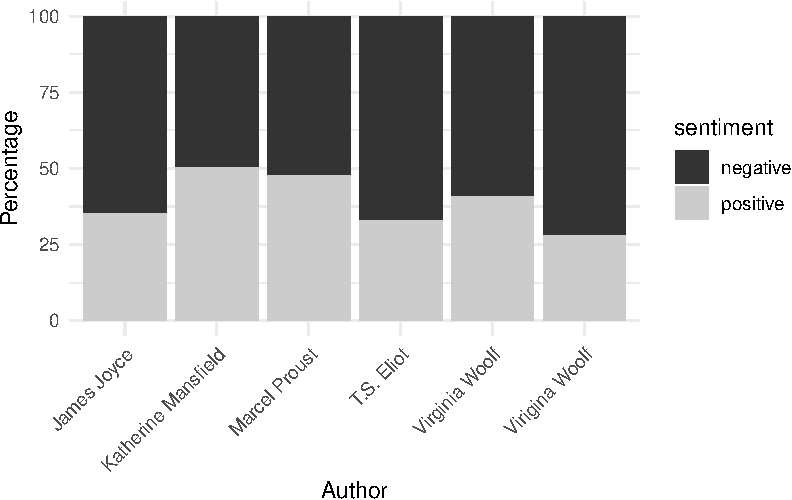
\includegraphics{paper_files/figure-pdf/fig-sentiment-1.pdf}

}

\caption{\label{fig-sentiment}Sentiment Analysis of All SOC Novels}

\end{figure}%

\begin{figure}

\centering{

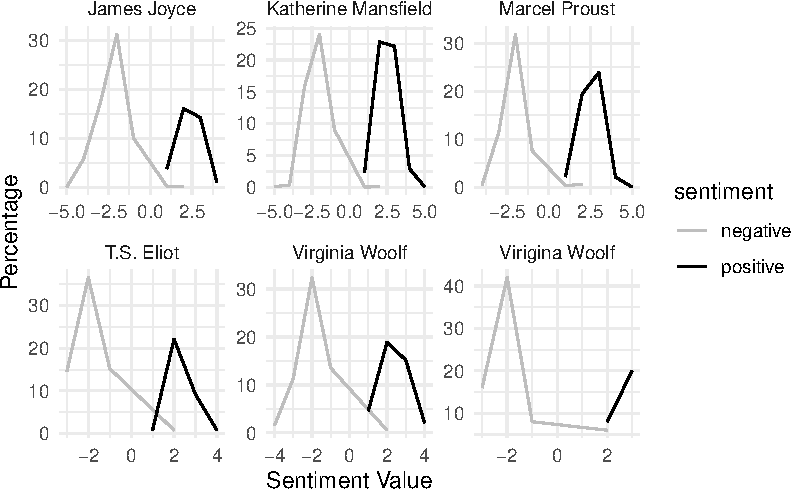
\includegraphics{paper_files/figure-pdf/fig-sentiment-number-1.pdf}

}

\caption{\label{fig-sentiment-number}Sentiment Analysis of All SOC
Novels by Sentiment Value}

\end{figure}%

\subsection{Gendered Mental Landscape of Stream of Consciousness
Novels}\label{gendered-mental-landscape-of-stream-of-consciousness-novels}

\begin{figure}

\begin{minipage}{0.50\linewidth}

\centering{

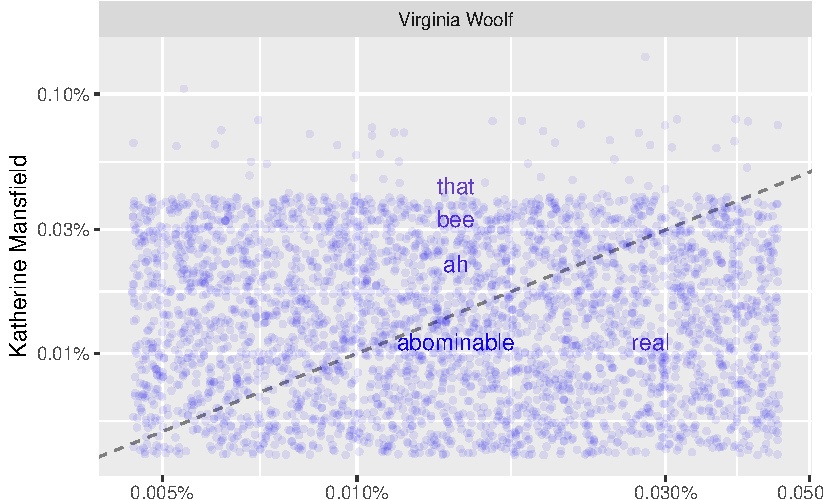
\includegraphics{paper_files/figure-pdf/fig-word-gender-1.pdf}

}

\subcaption{\label{fig-word-gender-1}Female Authors}

\end{minipage}%
%
\begin{minipage}{0.50\linewidth}

\centering{

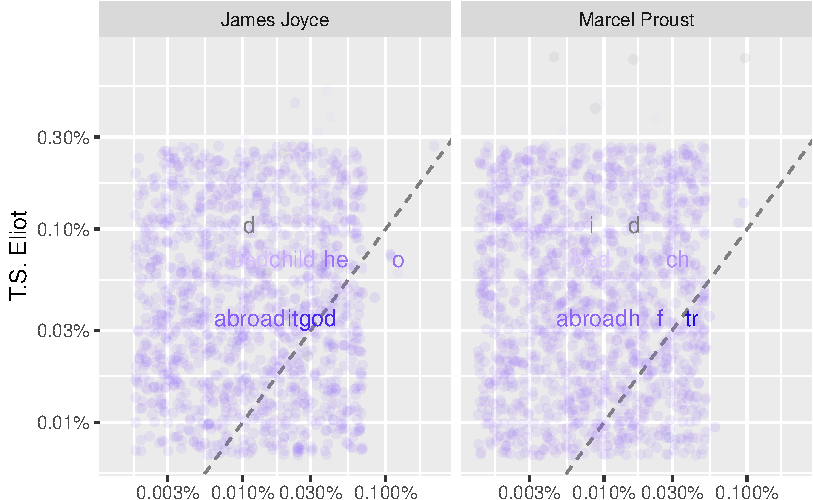
\includegraphics{paper_files/figure-pdf/fig-word-gender-2.pdf}

}

\subcaption{\label{fig-word-gender-2}Male Authors}

\end{minipage}%

\caption{\label{fig-word-gender}Comparative Analysis of Word Frequency
in Female and Male Stream of Consciousness Authors}

\end{figure}%

\subsubsection{Comparing SOC Literature's Female
Authors}\label{comparing-soc-literatures-female-authors}

\subsubsection{Comparing SOC Literature's Male
Authors}\label{comparing-soc-literatures-male-authors}

\subsection{Transnational SOC Novels and Mental Health
Themes}\label{transnational-soc-novels-and-mental-health-themes}

\begin{figure}

\centering{

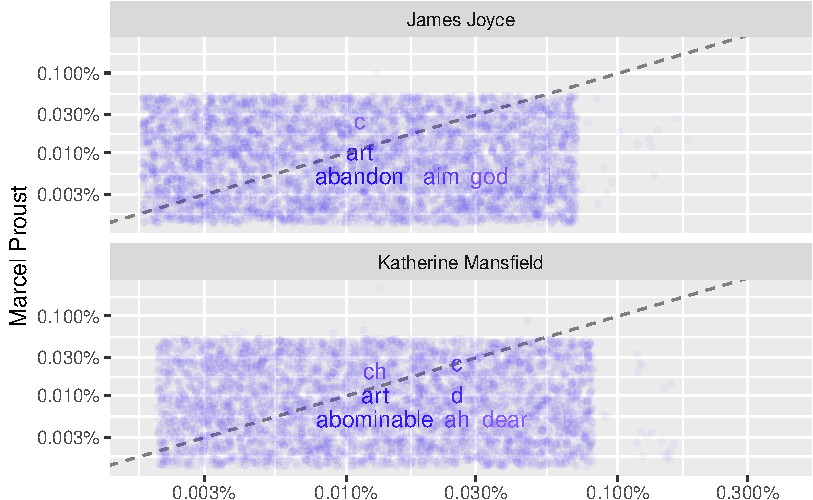
\includegraphics{paper_files/figure-pdf/fig-frequency-int-1.pdf}

}

\caption{\label{fig-frequency-int}Comparative Analysis of Word Frequency
in Transnational Stream of Consciousness Authors}

\end{figure}%

\newpage

\subsection{Combined Texts: Trends, Word Networks, Bigram and Trigram
Analsis}\label{combined-texts-trends-word-networks-bigram-and-trigram-analsis}

\begin{figure}

\begin{minipage}{0.50\linewidth}

\centering{

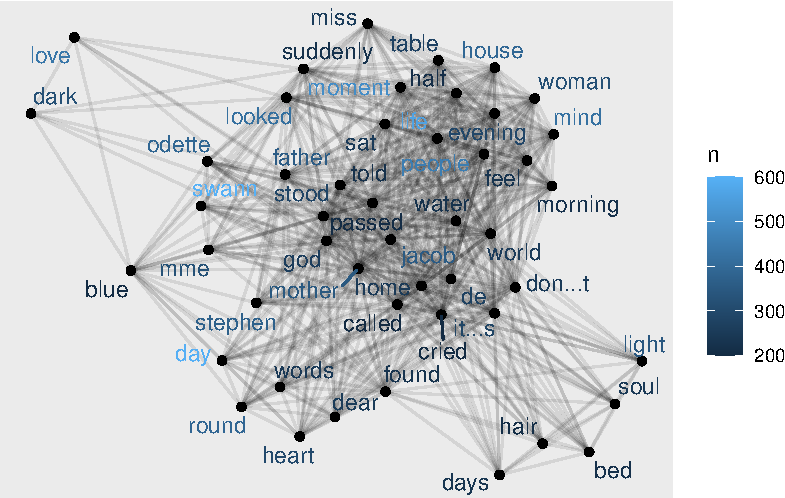
\includegraphics{paper_files/figure-pdf/fig-word-networks-1.pdf}

}

\subcaption{\label{fig-word-networks-1}100 Frequency, 0.2 Correlation}

\end{minipage}%
%
\begin{minipage}{0.50\linewidth}

\centering{

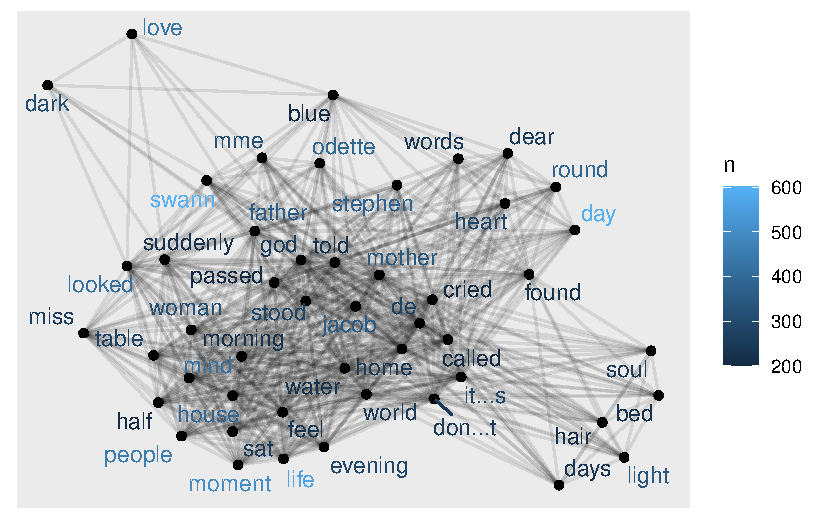
\includegraphics{paper_files/figure-pdf/fig-word-networks-2.pdf}

}

\subcaption{\label{fig-word-networks-2}200 Frequency, 0.4 Correlation}

\end{minipage}%
\newline
\begin{minipage}{0.50\linewidth}

\centering{

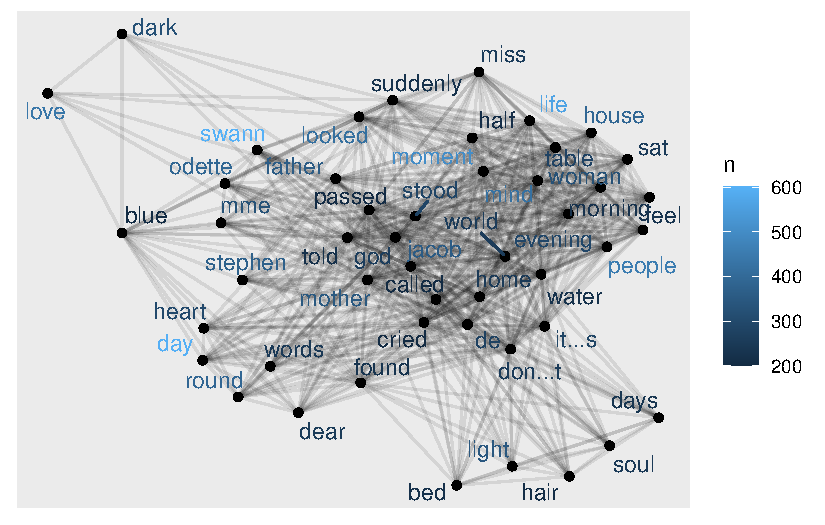
\includegraphics{paper_files/figure-pdf/fig-word-networks-3.pdf}

}

\subcaption{\label{fig-word-networks-3}200 Frequency, 0.8 Correlation}

\end{minipage}%
%
\begin{minipage}{0.50\linewidth}

\centering{

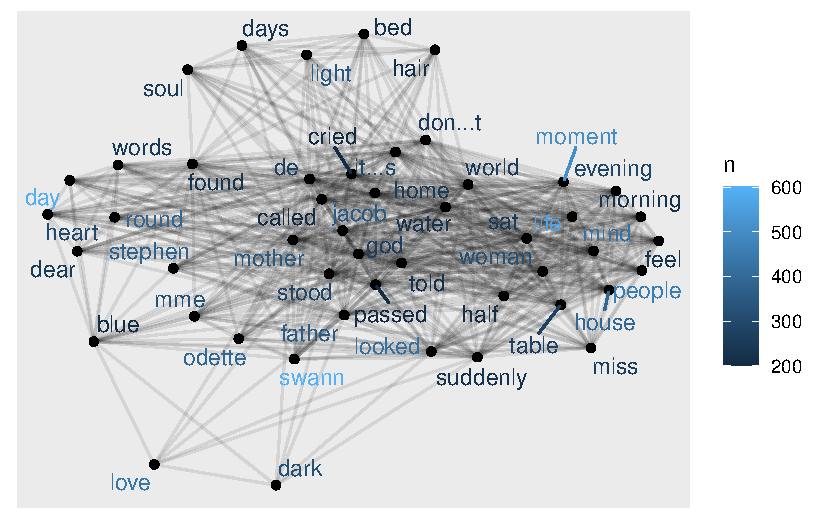
\includegraphics{paper_files/figure-pdf/fig-word-networks-4.pdf}

}

\subcaption{\label{fig-word-networks-4}400 Frequency, 1 Correlation}

\end{minipage}%

\caption{\label{fig-word-networks}Word Networks Measured by Frequency
and Correlation when Combining All Stream of Consciousness Novels}

\end{figure}%

\section{Discussion}\label{discussion}

\subsection{Mental Health Vocabulary: Patterns and
Trends}\label{mental-health-vocabulary-patterns-and-trends}

Discuss vocabulary patterns and word trends

\subsection{Insights into Socio-Political Landscape of the West's
Modernist
Era}\label{insights-into-socio-political-landscape-of-the-wests-modernist-era}

The novels' linguistic patterns reflect the socio-political landscape of
the Western hemisphere, from late 19th century to the mid-20th century.

\subsection{Schizophrenic and Disassociative Tendencies in Female Stream
of
Consciousness}\label{schizophrenic-and-disassociative-tendencies-in-female-stream-of-consciousness}

\subsection{Weaknesses}\label{weaknesses}

\subsubsection{Lack of Thorough Word
Cleaning}\label{lack-of-thorough-word-cleaning}

\subsubsection{Decontextualized Literature Works and Limiting
Publication
Editions}\label{decontextualized-literature-works-and-limiting-publication-editions}

\subsubsection{Uneven Novel Length and Categorization of
Authors}\label{uneven-novel-length-and-categorization-of-authors}

\subsubsection{Project Gutenberg's Focus on the
Canon}\label{project-gutenbergs-focus-on-the-canon}

\subsection{Moving Forward and Next
Steps}\label{moving-forward-and-next-steps}

\newpage

\section{Appendix}\label{appendix}

\subsection{Additional Data Details}\label{additional-data-details}

\begin{Shaded}
\begin{Highlighting}[]
\DocumentationTok{\#\#| eval: true}
\DocumentationTok{\#\#| echo: false}
\DocumentationTok{\#\#| message: false}
\DocumentationTok{\#\#| warning: false}
\CommentTok{\#combined\_books }
\end{Highlighting}
\end{Shaded}

\subsubsection{Data Gathering}\label{data-gathering}

\begin{Shaded}
\begin{Highlighting}[]
\DocumentationTok{\#\#| echo: false}
\DocumentationTok{\#\#| message: false}
\DocumentationTok{\#\#| label: tbl{-}reasons{-}strip{-}search}
\DocumentationTok{\#\#| tbl{-}cap:}
\end{Highlighting}
\end{Shaded}

\subsubsection{Data Cleaning}\label{data-cleaning}

\begin{Shaded}
\begin{Highlighting}[]
\DocumentationTok{\#\#| echo: false}
\DocumentationTok{\#\#| message: false}
\DocumentationTok{\#\#| label: tbl{-}items{-}strip{-}search}
\DocumentationTok{\#\#| tbl{-}cap: }
\end{Highlighting}
\end{Shaded}

\subsection{Model Details}\label{sec-model-details}

\subsection{Posterior predictive
check}\label{posterior-predictive-check}

\subsection{Diagnostics}\label{diagnostics}

\newpage

\section*{References}\label{references}
\addcontentsline{toc}{section}{References}

\phantomsection\label{refs}
\begin{CSLReferences}{1}{0}
\bibitem[\citeproctext]{ref-rMark}
Allaire, J., Y. Xie, C. Dervieux, J. McPherson, J. Luraschi, K. Ushey,
A. Atkins, et al. 2024. \emph{Rmarkdown: Dynamic Documents for r}. R
package version 2.26. \url{https://github.com/rstudio/rmarkdown}.

\bibitem[\citeproctext]{ref-resampling}
Bernini, M., and C. Fernyhough. 2022. {``Resampling (Narrative) Stream
of Consciousness: Mind Wandering, Inner Speech, and Reading as Reversed
Introspection.''} \emph{Modern Fiction Studies} 68 (4): 639--67.
https://doi.org/\url{https://doi.org/10.1353/mfs.2022.0045}.

\bibitem[\citeproctext]{ref-rTm}
Feinerer, I., K. Hornik, and D. Meyer. 2008. {``Text Mining
Infrastructure in r.''} \emph{Journal of Statistical Software} 25 (5):
1--54. \url{https://doi.org/10.18637/jss.v025.i05}.

\bibitem[\citeproctext]{ref-youtube2}
Henry, T. 2021. {``Https://Www.youtube.com/Watch?v=ae\_XVhjHd\_o.''}
\url{https://www.youtube.com/watch?v=ae_XVhjHd_o}.

\bibitem[\citeproctext]{ref-rTextdata}
Hvitfeldt, Emil. 2022. \emph{Textdata: Download and Load Various Text
Datasets}. \url{https://github.com/EmilHvitfeldt/textdata}.

\bibitem[\citeproctext]{ref-rGuten}
Johnston, Myfanwy, and David Robinson. 2023. \emph{Gutenbergr: Download
and Process Public Domain Works from Project Gutenberg}.
\url{https://docs.ropensci.org/gutenbergr/}.

\bibitem[\citeproctext]{ref-flow}
Long, H., and J. So R. 2016. {``Turbulent Flow: A Computational Model of
World Literature.''} \emph{Modern Language Quarterly} 77 (3): 345--67.
https://doi.org/\url{https://doi.org/10.1215/00267929-3570656}.

\bibitem[\citeproctext]{ref-sentiment}
Mohammad, Saif M., and Peter D. Turney. 2013. {``Crowdsourcing a
Word-Emotion Association Lexicon.''} \emph{Computational Intelligence}
29 (3): 436--65. \url{https://doi.org/10.1111/j.1467-8640.2012.00460.x}.

\bibitem[\citeproctext]{ref-rHere}
Müller, Kirill. 2020. \emph{Here: A Simpler Way to Find Your Files}.
\url{https://CRAN.R-project.org/package=here}.

\bibitem[\citeproctext]{ref-pathology}
Nyongesa, A. 2023. {``The Centre and Pathology: Postmodernist Reading of
Madness in the Oppressor in Contemporary Fiction.''} \emph{Cogent Arts
\& Humanities} 10 (1): 1--12.
https://doi.org/\url{https://doi.org/10.1080/23311983.2023.2249280}.

\bibitem[\citeproctext]{ref-rGg}
Pedersen, L., T. 2024. \emph{Ggraph: An Implementation of Grammar of
Graphics for Graphs and Networks}.
\url{https://ggraph.data-imaginist.com}.

\bibitem[\citeproctext]{ref-gutenberg}
{``Project Gutenberg.''} n.d. \url{https://www.gutenberg.org}.

\bibitem[\citeproctext]{ref-r}
R Core Team. 2022. \emph{R: A Language and Environment for Statistical
Computing}. Vienna, Austria: R Foundation for Statistical Computing.
\url{https://www.R-project.org/}.

\bibitem[\citeproctext]{ref-citeR}
---------. 2023. \emph{R: A Language and Environment for Statistical
Computing}. Vienna, Austria: R Foundation for Statistical Computing.
\url{https://www.R-project.org/}.

\bibitem[\citeproctext]{ref-youtube1}
Robertson, C. 2021. {``Text Tokenization in r.''}
\url{https://www.youtube.com/watch?v=9T-hr3jinTw}.

\bibitem[\citeproctext]{ref-rIgraph}
Silge, J., and D. Robinson. 2006. {``The Igraph Software Package for
Complex Network Research.''} \emph{InterJournal,*Complex Systems*},
1695. \url{https://igraph.org}.

\bibitem[\citeproctext]{ref-rWidy}
---------. 2022. \emph{Widyr: Widen, Process, Then Re-Tidy Data}.
\url{https://github.com/juliasilge/widyr}.

\bibitem[\citeproctext]{ref-rTidytext}
Silge, Julia, and David Robinson. 2016. {``Tidytext: Text Mining and
Analysis Using Tidy Data Principles in r.''} \emph{JOSS} 1 (3).
\url{https://doi.org/10.21105/joss.00037}.

\bibitem[\citeproctext]{ref-rGgplot2}
Wickham, Hadley. 2016. \emph{Ggplot2: Elegant Graphics for Data
Analysis}. Springer-Verlag New York.
\url{https://ggplot2.tidyverse.org}.

\bibitem[\citeproctext]{ref-rTidyverse}
Wickham, Hadley, Mara Averick, Jennifer Bryan, Winston Chang, Lucy
D'Agostino McGowan, Romain François, Garrett Grolemund, et al. 2019.
{``Welcome to the {tidyverse}.''} \emph{Journal of Open Source Software}
4 (43): 1686. \url{https://doi.org/10.21105/joss.01686}.

\bibitem[\citeproctext]{ref-rDplyr}
Wickham, Hadley, Romain François, Lionel Henry, and Kirill Müller. 2022.
\emph{Dplyr: A Grammar of Data Manipulation}.
\url{https://CRAN.R-project.org/package=dplyr}.

\bibitem[\citeproctext]{ref-rScales}
Wickham, Hadley, Thomas Lin Pedersen, and Dana Seidel. 2023.
\emph{Scales: Scale Functions for Visualization}.
\url{https://scales.r-lib.org}.

\bibitem[\citeproctext]{ref-rKnitr}
Xie, Yihui. 2014. {``Knitr: A Comprehensive Tool for Reproducible
Research in {R}.''} In \emph{Implementing Reproducible Computational
Research}, edited by Victoria Stodden, Friedrich Leisch, and Roger D.
Peng. Chapman; Hall/CRC.
\url{http://www.crcpress.com/product/isbn/9781466561595}.

\end{CSLReferences}



\end{document}
